% Created 2022-06-10 Fri 17:31
% Intended LaTeX compiler: pdflatex
\documentclass[letter,11pt,twocolumn]{extarticle}
\usepackage[utf8]{inputenc}
\usepackage[T1]{fontenc}
\usepackage{graphicx}
\usepackage{longtable}
\usepackage{wrapfig}
\usepackage{rotating}
\usepackage[normalem]{ulem}
\usepackage{amsmath}
\usepackage{amssymb}
\usepackage{capt-of}
\usepackage{hyperref}
\usepackage[bitstream-charter]{mathdesign}
\usepackage[left=1in,right=1in]{geometry}
\usepackage{tikz-cd}
\usetikzlibrary{cd}
\setlength{\columnsep}{0.3in}
\author{Yuan Fu \\yuf011@ucsd.edu \and Linfang He \\ l8he@ucsd.edu \and Xuanzhu Zhou \\ xuz004@ucsd.edu \and in alphabetical order}
\date{\today}
\title{File Sharing with 0 Responsibility}
\hypersetup{
 pdfauthor={Yuan Fu},
 pdftitle={File Sharing with 0 Responsibility},
 pdfkeywords={},
 pdfsubject={},
 pdfcreator={Emacs 29.0.50 (Org mode 9.5.2)}, 
 pdflang={English}}
\begin{document}

\maketitle

\section{Abstract}
\label{sec:org793cd85}

We present a distributed network FUSE filesystem to support personal/family file sharing. Our system gives up on strong consistency to maximize availability and simplicity. Our system is able to savage files even when the owner of the file is offline, and employs major-minor versioning to reduce write conflicts. We are able to implement our system in a short amount of time and verify its correctness.

\section{Introduction}
\label{sec:org2ed71f7}

In this report we present a distributed FUSE filesystem aimed at personal/family file sharing between multiple hosts. We have a certain set of goals when designing the system: We want to maximize the availability for our system. We want to maximize the simplicity of our system, for both the virtue of simplicity itself and the limit in resources. And we want our system to be reasonably simply to use, but without hiding too much details so that users cannot easily understand it or control it.

These goals are derived from our dissatisfaction of contemporary network filesystems like iCloud, Dropbox, SSHFS, etc. They either gives user little control over the system, or assumes network is always connected \footnote{Which is a horrible assumption to be made when one is on UCSD campus.}, or does not integrate with local file system transparently.

In return of availability and simplicity, we give up some consistency of our system, opportunistically assume bad things rarely happen. This assumption isn’t unreasonable to take as our target usecase is single-user or faimily file sharing, meaning the number of hosts is small, files updates are occasional, and conflicting modifications are rare.

In our setting, each host has a local “vault”, in which is stores and owns some files. This host wants to access other hosts vault, and want to share files its own vault to others. All of the hosts combine their vaults into a filesystem, in which each vault is a direct subdirectory of the filesystem root. This filesystem is mounted on each host.

There has been abundant prior work on a distributed filesystem, including Coda \cite{10.1145/146941.146942}, Bayou \cite{10.1145/224057.224070}, and SSHFS \cite{10.5555/1134782.1134786}. Coda makes the distinction between first-class servers and second-class clients. We take an approach closer to Bayou, where there is no distinction of server and client. But under the hood, each host act as the server of its local vault, which it owns and manages. Other hosts’s local copy of this vault succumbs should conflict with the owner of the vault arises.

Unlike Bayou, which relies on application to provide a semantic for resolving conflict, our system provides an ordinary filesystem interface and doesn’t resolve file conflicts automatically.

SSHFS focuses on conveniently mounting a remote machine through SSH, and doesn’t provide good disconnection operation. It doesn’t interconnect multiple hosts mutually, either.

The main interesting bit of our system, comparing to Coda, is its ability to “savage“ files: when a host Alice is not connected, a host Bob could savage files owned by Alice from Charlie, if Charlie has previously accessed that file and cached it. Our versioning system complements savaging, and uses a major version plus a minor version. This versioning system allows us to perverse more work when resolving conflict.

\section{Design overview}
\label{sec:org237f099}

In this section we describe the high-level design of our system, the operational semantic it provides, and compare our semantic to that of Coda and Bayou.

\subsection{High-level overview}
\label{sec:org38c2d6f}

As we previously described, each host possess a local vault that it owns and shares, and all hosts’ vault combines into a global filesystem that is mounted onto each host. An example is shown in \ref{fig:global_filesystem}.

\begin{figure}
\begin{center}
% https://q.uiver.app/?q=WzAsNCxbMSwwLCIvIl0sWzAsMSwiQWxpY2UiXSxbMSwxLCJCb2IiXSxbMiwxLCJDaGFybGllIl0sWzAsMV0sWzAsMl0sWzAsM11d
\begin{tikzcd}
	& {/} \\
	Alice & Bob & Charlie
	\arrow[from=1-2, to=2-1]
	\arrow[from=1-2, to=2-2]
	\arrow[from=1-2, to=2-3]
\end{tikzcd}
\end{center}
\label{fig:global_filesystem}
\caption{In a system with three hosts, Alice, Bob, and Charlie, the file system contains all three of their vaults.}
\end{figure}

On each host, access to the local vault is handled locally, and access to other vaults are translated to requests to the remote host that owns that vault. In the same time, the local host serves requests from other hosts for contents in its local vault.

To maximize availability, the local filesystem instance caches remote content and substitute for the remote vault in case of disconnection. And during normal operation when the remote vault is connected, the local filesystem “hoards” files preemptively, so that a future disconnect does not stop the user from accessing the files. During disconnection, if the user requests for a file that the filesystem didn’t hoard, the filesystem still tries its best by “savaging” for that file from other connected hosts—maybe they have hoarded it. This is different from Coda, which assumes a client is either connected to the servers (and thus can access all the files) or not.

In order to keep the system simple, we do not allow file ownership to migrate, the owner of the vault manages that vault, and everyone else contacts the owner to modify the file or metadata in that vault. The owner is the serialization point and the source-of-truth. When the owner cannot be contacted, other host simply holds onto their modification until the owner is online again.

\subsection{Semantics}
\label{sec:org434a0a1}

We provide a subset of the functionality normally provided by a filesystem. Notable omissions include flush(), permissions, hard links, renaming, append mode and read-only mode. Below we discuss the semantics of representative operations in connected and disconnected contexts for remote files.

When connected, file operations on remote files have the following semantics:

\begin{description}
\item[{open}] Successfully opening a file downloads the whole file to a local copy, meaning following read and write does not fail even if the remote vault loses contact.
\item[{read}] Reading a remote file reads the local copy of the file rather than the latest version available on the remove vault, even if the local filesystem is connected to the remote vault. This means other concurrent access to the same file can affect the process using that file, similar to other UNIX filesystems.
\item[{write}] Similar to read, write only writes to the local copy and the change is not guaranteed to persist.
\item[{close}] Successfully closing a file ensures the modification are written to local disk and thus persists (until another process overwrites it). But there is no guarantee that this version will be accepted by the owner. Closing a modified file increments its version.
\item[{getattr}] Operations that retrieve metadata like lookup(), open(), readdir(), getattr() directly contacts the remote vault for metadata when connection is up. That is, they reflect the current state of the remote vault at time of operation. It is possible that a file is deleted remotely before it is closed locally. In that case, just like conventional UNIX filesystem, the process opened the file can still read and write the file before closing it, and other processes cannot open that file anymore.
\item[{create/delete}] Operations that modifies metadata like setattr(), create(), mkdir(), rmdir(), unlink() directly contacts the remote vault when connection is up.
\end{description}

Overall, operations when connected are less interesting and we provide similar semantics to Coda and Bayou. Both Coda and our system fetches the whole file on open.

When disconnected, meaning the owner of the vault lost contact, the semantics is slightly different:

\begin{description}
\item[{open}] If a local copy exists, that version is used, even if other connected hosts has newer versions, because we assume such condition is rare. If a local copy does not exist, the filesystem tries to find a copy from other connected hosts, we call this process “savage”. If no one has a copy, the filesystem returns an error\footnote{We decide to return ENETDOWN rather than ENOENT. This is a relatively arbitrary decision, we think either choice makes sense and this choice could be user-configurable.}. We discuss the consistency implication of savaging below.
\item[{read/write}] Disconnected read and write are the same as connected one, if the process is able to open the file. Otherwise it can’t read nor write.
\item[{close}] Closing the file during disconnection actually has the same semantics as when connected: changes are persisted locally on disk, but there is no guarantee that the owner accepts the change.
\item[{getattr}] During disconnection, metadata query are handled by the local cache. The cache reflect the value of the last successful remote metadata query, because that is when this information is cached. Generally the metadata is fully hoarded as they don’t take much space.
\item[{delete}] Disconnect metadata modification is handled similarly to Coda. The local filesystem applies the change locally and returns immediately. It also keeps a log of all local operations, and tries to replay it once the remote vault is connected again. A conflict during replay (including file modification and metadata modification) does not abort the process, unlike in Coda. We try to be maximally opportunistic and merge as much change as possible.
\item[{create}] Currently we don’t support creating new files and directories during disconnection. We plan to add this feature in the future.
\end{description}

During disconnection, Coda only consults the local cache, while our system savages for the file from other connected hosts. After all, it doesn’t make much sense to not provide service if there is a copy and we can access it. In this sense we are closer in spirit to Bayou. We handle conflicts similar to Coda, i.e., we make reasonable effort in the range of our ability—even though that range is rather limited due to the primitive interface we expose. Bayou can do significantly more, at the cost of requiring more involvement from applications.

\subsection{Maximally opportunistic and minimally responsible}
\label{sec:orgebdc731}

Because we assume conflicts rarely happen and most hosts are connected to each other most of the time, and we try to maximize availability and simplicity, our system makes minimum effort on enforcing consistency.

For example, when the owner is disconnected and we have a local copy, we do not check for more recent copied that could exist on other connected hosts. This decision is made because we assume most hosts are mostly connected, and thus most of the time the local copy is the up-to-date version. By not querying other hosts, we can serve the user immediately.

When savaging, we return with the first copy we find. Because, again, we assume most likely everybody has the most up-to-date version.

Coda tries to save user’s work and spits out diffs when reintegration failed, we don’t even try to do that. If a version lost a race, it is gone—next open fetches the remote version. If a remote host made changes to files in the local vault and submitted the change, the local file is immediately overwritten, even if some process are accessing it. We made this decision to simplify our implementation and we assume such conflicts rarely happens in the use-case of our system. If a user wants more safety, they can use version control system and auto-backup features available on most text editors.

\begin{figure}
% https://q.uiver.app/?q=WzAsOSxbNCwxLCJmIl0sWzQsMCwiXFx0ZXh0e0FsaWNlfSJdLFsyLDEsImYiXSxbMiwwLCJcXHRleHR7Qm9ifSJdLFsyLDIsImYnIl0sWzAsMiwiZiciXSxbMCwwLCJDaGFybGllIl0sWzAsMywiZicnIl0sWzQsNCwiPyJdLFswLDJdLFsyLDRdLFs0LDVdLFs1LDddLFs3LDhdLFs0LDhdXQ==
\begin{tikzcd}
	Charlie && {\text{Bob}} && {\text{Alice}} \\
	&& f && f \\
	{f'} && {f'} \\
	{f''} \\
	&&&& {?}
	\arrow[from=2-5, to=2-3]
	\arrow[from=2-3, to=3-3]
	\arrow[from=3-3, to=3-1]
	\arrow[from=3-1, to=4-1]
	\arrow[from=4-1, to=5-5]
	\arrow[from=3-3, to=5-5]
\end{tikzcd}
\caption{Bob fetches from Alice, Charlie savages from Bob. When Alice comes back online, either Bob’s or Charlie’s version could win.}
\label{fig:race}
\end{figure}

\subsection{Versioning and conflict resolution}
\label{sec:orge7d8d29}

The addition of savaging brings an interesting case into conflict resolution. Consider such a scenario (illustrated in figure \ref{fig:race}): host Alice has a file \(f\), which host Bob fetched and cached. Then Alice goes offline, and Bob makes some changes to \(f\) to become \(f'\). Now host Charlie tries to fetch \(f\) from Alice but couldn’t, and savages \(f'\) from Bob. Charlie proceed to change \(f'\) to \(f''\). Now Alice is back online, Bob and Charlie both race to submit their version to Alice. One of the output is actually better than the other: If Charlie wins, both his and Bob’s work are submitted; but if Bob wins, Charlie’s work cannot be submitted to Alice and he has to manually resolve the conflict.

We designed our versioning system such that Charlie always win. Specifically, we allow Charlie’s version to overwrite Bob’s, but not the other way around.

We model fetching, savaging and submitting files as a directed acyclic graph: fetching and savaging are modeled as a fork, and submitting a merge. A version consists of a major version number and a minor version number. The first change to a file after a fork or merge bumps the major version number, and all subsequent changes only bumps the minor version number, until next fork or merge. Merging and forking operations don’t change the version.

Figure \ref{fig:versioning} gives an example of forking and merging: Bob forks a file at version 1.0 from Alice, the first change to the file bumps it to version 2.0. Then Charlie forks the file from Bob. Both Bob’s and Charlie’s next change to the file bumps the version to 3.0. Bob proceeds to make another change and brings the version to 3.1. Charlie made two changes and brings the version to 3.2. Then Dave forks from Charlie, so Charlie’s and Dave’s next change bumps the version to 4.0.

When Alice comes online, Bob’s submits version 3.1 first and succeeds. Then Charlie submits his version 4.0 and succeeds, overwriting Bob’s version. Dave’ tries to submit version 4.0 but fails.

An interesting implication of this version system is that, having your version forked by other hosts, like Charlie had, increases your chance of winning and preserving your work. This is desirable because we want the version most people hold to win.

Note that when the owner (Alice in our example) can be contacted, our system do not bother to query other hosts for newer versions, because we assume that if the owner is online, any change made by other hosts are promptly submitted back to the owner, and there is no need to query all the hosts.

\begin{figure}
% https://q.uiver.app/?q=WzAsMTksWzAsMCwiXFx0ZXh0e0FsaWNlfSJdLFsxLDAsIlxcdGV4dHtCb2J9Il0sWzIsMCwiXFx0ZXh0e0NoYXJsaWV9Il0sWzMsMCwiXFx0ZXh0e0RhdmV9Il0sWzAsMSwiMS4wIl0sWzEsMSwiMS4wIl0sWzEsMiwiMi4wIl0sWzEsMywiMy4wIl0sWzIsMywiMy4wIl0sWzEsNCwiMy4xIl0sWzIsNCwiMy4xIl0sWzIsNSwiMy4yIl0sWzMsNSwiMy4yIl0sWzIsNiwiNC4wIl0sWzAsNCwiMy4xIl0sWzAsNiwiNC4wIl0sWzIsMiwiMi4wIl0sWzMsNywiNC4wIl0sWzAsNywiXFx0aW1lcyJdLFs0LDVdLFs1LDZdLFs2LDddLFs3LDldLFs4LDEwXSxbMTAsMTFdLFsxMSwxM10sWzksMTRdLFsxMywxNV0sWzExLDEyXSxbNiwxNl0sWzE2LDhdLFsxMiwxN10sWzE3LDE4XV0=
\begin{tikzcd}
	{\text{Alice}} & {\text{Bob}} & {\text{Charlie}} & {\text{Dave}} \\
	{1.0} & {1.0} \\
	& {2.0} & {2.0} \\
	& {3.0} & {3.0} \\
	{3.1} & {3.1} & {3.1} \\
	&& {3.2} & {3.2} \\
	{4.0} && {4.0} \\
	\times &&& {4.0}
	\arrow[from=2-1, to=2-2]
	\arrow[from=2-2, to=3-2]
	\arrow[from=3-2, to=4-2]
	\arrow[from=4-2, to=5-2]
	\arrow[from=4-3, to=5-3]
	\arrow[from=5-3, to=6-3]
	\arrow[from=6-3, to=7-3]
	\arrow[from=5-2, to=5-1]
	\arrow[from=7-3, to=7-1]
	\arrow[from=6-3, to=6-4]
	\arrow[from=3-2, to=3-3]
	\arrow[from=3-3, to=4-3]
	\arrow[from=6-4, to=8-4]
	\arrow[from=8-4, to=8-1]
\end{tikzcd}
\caption{Bob forks from Alice, Charlie forks from Bob, Dave forks from Charlie. The first change after a fork bumps the major version, subsequent changes bump the minor version. The version with a larger major version wins a conflict; if the major version is the same, the first submission wins the conflict.}
\label{fig:versioning}
\end{figure}

\subsection{Replication}
\label{sec:org5c72ef2}

Replication comes for free from the combination of savaging and hoarding. If a user wants to replicate some files, they can explicitly instruct the filesystem to hoard them on multiple hosts. We currently have not implemented explicit hoarding but plan to in the future.

We don’t think automatically replicating all the files makes much sense in our settings. Home computers usually have limited storage and hard disk failure is generally not a concern.

\begin{figure*}
\begin{center}
\begin{tikzcd}[sep=small]
	userspace &&&& {\text{RemoteVault}} \\
	& LocalVault &&& \vdots \\
	&& VaultServer && {\text{RemoteVault}} \\
	FUSE & RemoteVault &&& {\text{RemoteVault}} & {\text{FUSE}} \\
	& RemoteVault && {\text{VaultServer}} \\
	& \vdots &&& {\text{LocalVault}} && {} \\
	& RemoteVault &&&& {\text{userspace}}
	\arrow[from=1-1, to=4-1]
	\arrow[bend left=30, from=4-1, to=2-2]
	\arrow[from=4-1, to=4-2]
	\arrow[from=3-3, to=2-2]
	\arrow["rpc", dashed, from=4-5, to=3-3]
	\arrow[from=5-4, to=6-5]
	\arrow["rpc"', dashed, from=4-2, to=5-4]
	\arrow[from=4-6, to=4-5]
	\arrow[bend left=30, from=4-6, to=6-5]
	\arrow[from=7-6, to=4-6]
	\arrow[from=3-3, to=4-2]
	\arrow[from=5-4, to=4-5]
	\arrow[bend right=30, from=4-1, to=5-2]
	\arrow[bend right=30, from=4-6, to=3-5]
	\arrow[bend right=30, from=4-1, to=7-2]
	\arrow[bend right=30, from=4-6, to=1-5]
	\arrow[from=3-3, to=5-2]
	\arrow[from=3-3, to=7-2]
	\arrow[from=5-4, to=3-5]
	\arrow[from=5-4, to=1-5]
\end{tikzcd}
\end{center}
\caption{Two monovault instances typed in italics and roman, respectively. Arrows go in the direction of requests. Dashed arrows represent rpc requests over the network.}
\label{fig:modules}
\end{figure*}

\section{Implementation}
\label{sec:org1bad070}
\subsection{Modularization}
\label{sec:org36a2100}

In this section we introduce our design details. We compartmentalized our system into modules, each providing service to each other. Figure \ref{fig:modules} demonstrates the interaction between each modules and between monovault instances. The FUSE module implements the FUSE API and provides service to the userspace. It delegates requests to each vault modules. A vault module can be either a local vault which stores files locally or a remote vault module that sends requests through rpc to remote hosts and (optionally) caches copies locally.

Each monovault instance also runs a vault server than handles requests from other hosts. Similar to the FUSE module, it delegates requests to the vault modules. Normally the server only delegate requests to the local vault modules, which serves the local vault. A vault server occasionally delegate request to a remote vault instance—that’s when its client are savaging for files.

\subsection{FUSE module}
\label{sec:org461df8e}

One interesting tasks that the FUSE module performs is to translate inode numbers. In our system, files are identified by inode numbers. Each vault uses its own independent number space for inode numbers. Therefore, to combine multiple vaults under a single file system and not have inode number conflicts, the FUSE layer translates between vault-local inode numbers and global inode numbers. Specifically, a 64 bit global inode number is split into a 16 bit prefix and a 48 bit body. Each vault is assigned a 16 bit prefix and gets 48 bits of local inode number space. The global inode is then simply the 16 bit prefix concatenated with the 48 bit local inode.

Note that the “global“ inode number is not a global consensus between all the hosts. Rather, it is only visible to the userspace and is ephemeral to the host—upon restart, the filesystem could give each vault a different prefix. It is only used for accommodating individual vaults under a single filesystem.

\subsection{Vaults}
\label{sec:org52afc01}

Figure \ref{fig:vaults} illustrates the flow of requests from the FUSE module to LocalVault and CachingRemote module on the other host. We explain below what does each module does.

\begin{description}
\item[{LocalVault}] The local vault needs to manage two things: file data and file metadata. File data are simply stored in the filesystem of the host OS as individual files. Metadata are recorded and managed in a SQLite database. When a file is recorded in the database, its data file must exist on disk. Directories live entirely in the database and have no associated data files.

\item[{VaultServer}] The vault server runs in the background and serves rpc requests from remote hosts. For requests on the local vault, it simply delegates the request to the local vault. Savage requests are delegated to remote vaults.

\item[{RemoteVault}] A remote client is an abstraction over direct and caching remote vault clients. \textbf{DirectRemote} simply turns FUSE requests into rpc requests, while \textbf{CachingRemote} performs interesting operations like savaging and caching. CachingRemote can serve savage requests because they have cache, DirectRemotes cannot.

\item[{BackgroundWorker}] All write requests are sent to the background worker and the main thread can return immediately. BackgroundWorker runs in a independent thread and sends write and submit requests to the remote server in the background.
\end{description}

\begin{figure*}
\begin{center}
% https://q.uiver.app/?q=WzAsOCxbMCw3LCJcXHRleHR7RGlyZWN0UmVtb3RlfSJdLFsyLDcsIlxcdGV4dHtDYWNoaW5nUmVtb3RlfSJdLFsxLDIsIlxcdGV4dHtWYXVsdFNlcnZlcn0iXSxbMCwwLCJcXHRleHR7TG9jYWxWYXVsdH0iXSxbMiwwLCJcXHRleHR7Q2FjaGluZ1JlbW90ZX0iXSxbMSw0LCJcXHRleHR7UnBjQ2xpZW50fSJdLFsxLDksIlxcdGV4dHtGVVNFfSJdLFsxLDYsIlxcdGV4dHtCYWNrZ3JvdW5kV29ya2VyfSJdLFsyLDQsInNhdmFnZSIsMV0sWzIsMywicmVhZCx3cml0ZSxzdWJtaXQsc2F2YWdlIiwxXSxbMSw1LCJzYXZhZ2UiLDFdLFswLDUsInJlYWQiLDFdLFs1LDIsInJwYyIsMSx7InN0eWxlIjp7ImJvZHkiOnsibmFtZSI6ImRhc2hlZCJ9fX1dLFs2LDBdLFs2LDFdLFs3LDUsIndyaXRlLHN1Ym1pdCIsMV0sWzEsNywic3VibWl0IiwxXSxbMCw3LCJ3cml0ZSIsMV1d
\begin{tikzcd}
	{\text{LocalVault}} && {\text{CachingRemote}} \\
	\\
	& {\text{VaultServer}} \\
	\\
	& {\text{RpcClient}} \\
	\\
	& {\text{BackgroundWorker}} \\
	{\text{DirectRemote}} && {\text{CachingRemote}} \\
	\\
	& {\text{FUSE}}
	\arrow["savage"{description}, from=3-2, to=1-3]
	\arrow["{read,write,submit,savage}"{description}, from=3-2, to=1-1]
	\arrow["savage"{description}, from=8-3, to=5-2]
	\arrow["read"{description}, from=8-1, to=5-2]
	\arrow["rpc"{description}, dashed, from=5-2, to=3-2]
	\arrow[from=10-2, to=8-1]
	\arrow[from=10-2, to=8-3]
	\arrow["{write,submit}"{description}, from=7-2, to=5-2]
	\arrow["submit"{description}, from=8-3, to=7-2]
	\arrow["write"{description}, from=8-1, to=7-2]
\end{tikzcd}
\end{center}
\caption{The dierct and caching remote on the bottom receives requests from the FUSE modules and sends requests to the remote vault server through rpc. Direct remote sends read and write requests, caching remote sends savage and submit requests. Write and submit requests are sent asynchronisely by BackgroundWorker. On the other side, VaultServer uses LocalVault and CachingRemote to serve requests.}
\label{fig:vaults}
\end{figure*}

\subsection{The hoarder}
\label{sec:orgcee3aa6}

The hoarder is simply another thread that walks the directory tree of each vault and stores all the metadata locally. Due to limited time, we didn’t implement hoarder.

\subsection{Interfaces}
\label{sec:org334f44e}

The interface provided by LocalVault, and RemoteVault is as follows:

\begin{verbatim}
attr(file)
read(file, offset, size)
write(file, offset, data)
create(parent, name, type)
open(file)
close(file)
delete(file)
readdr(dir)
\end{verbatim}

Our rpc interface contains all the functions above, plus:

\begin{verbatim}
savage(vault, file)
submit(file, version)
\end{verbatim}

\section{Evaluation}
\label{sec:org6a226fa}

In this section we evaluate the correctness of our system. We are able to verify that features like offline editing, hoarding (if you implemented it), savaging and versioned conflict resolution works as we intended.

\subsection{Experimentation setup}
\label{sec:org58689dc}

The tests are conducted on macOS with Apple M1 chip and 16 GB main memory. The version of rust is rustc 1.59.0 (9d1b2106e 2022-02-23) and the version of fuse is macFUSE 4.2.5.

\subsection{Offline editing}
\label{sec:org4ce84b5}

For the first test, we have two clients Alice and Bob which are initially connected, so they can both read and write each other’s files. Then Bob is disconnected and Alice modifies file “f1” by adding a few lines. We expect that when Bob is back to connection, the modification by Alice can be synced with client Bob. The graph below also described the process.

\begin{center}
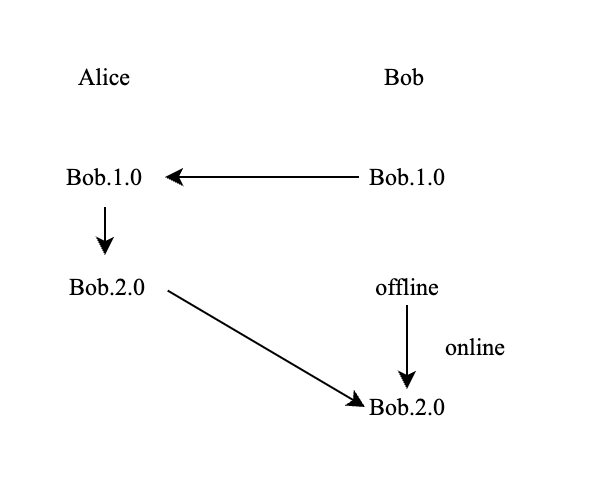
\includegraphics[width=.9\linewidth]{./evaluation/1.png}
\end{center}

We found that the modification can be successfully synchronized.

\subsection{Savaging}
\label{sec:orgb3ecc31}

For the second test, we have three clients Alice,Bob, and Charlie which are all initially connected. Charlie read one of Bob’s file “f2” before Bob becomes disconnected. Then Alice tries to read file “f2”. We expect this operation to be successful because Alice can read this file from Charlie who has cached file “f2” from Bob. The graph below describes the process.

\begin{center}
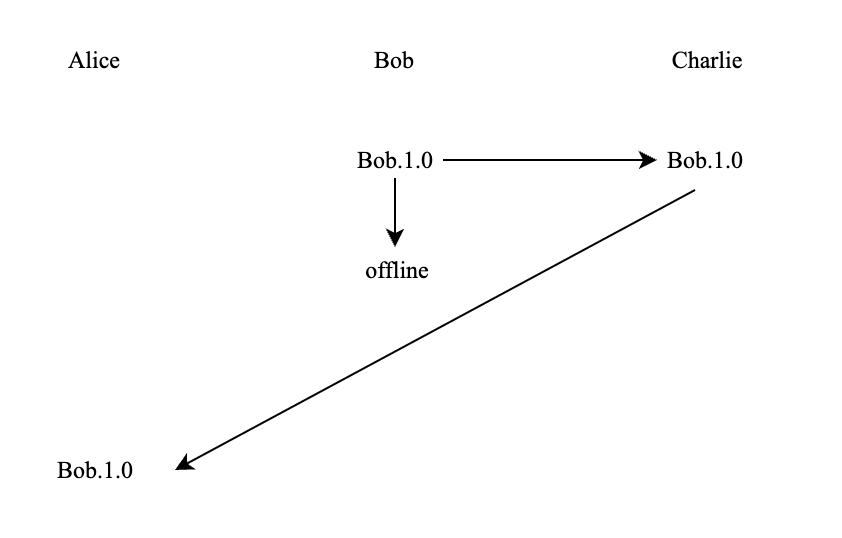
\includegraphics[width=.9\linewidth]{./evaluation/2.png}
\end{center}

We found that Alice can successfully read file “f2”.

\subsection{Versioning and conflict resolution}
\label{sec:orgf8260bf}

For the third test, we have three clients Alice, Bob, and Charlie which are all initially connected. Bob read one of A’s file “f3” and made some modifications before Alice becomes disconnected. Then Charlie reads file “f3” from Bob and also makes some modification. At last, all three clients are connected back together. We expect file “f2” in Alice to contain modifications made by Charlie.
The graph below describes the process.

\begin{center}
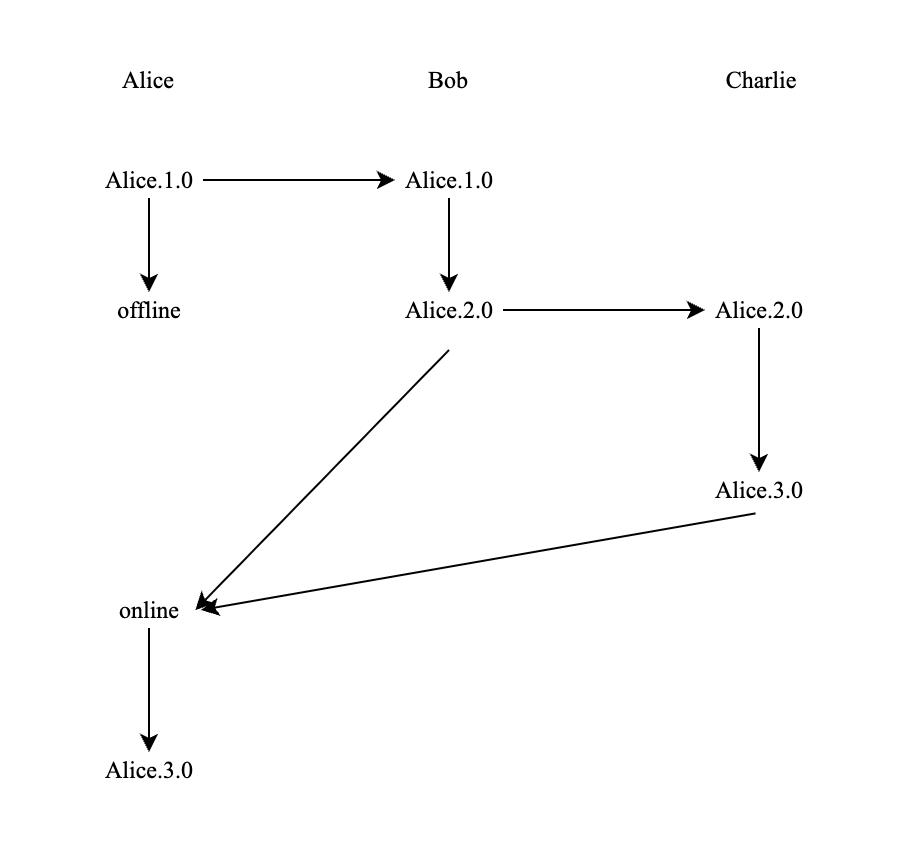
\includegraphics[width=.9\linewidth]{./evaluation/3.png}
\end{center}

We found that the the file “f2” in Alice contains modifications made by Charlie.

\section{Future work}
\label{sec:org0bad79d}

Due to time constraint, we are unable to implement some features that a sensible filesystem ought to have. We consider them future work.

\subsection{More efficient file transfer}
\label{sec:orgcd0c8b6}

Currently in savage and submit requests we send the whole file. In the future we plan to incorporate more efficient ways, like the rsync algorithm \cite{1885-40765}.

\subsection{Updating atime and mtime of directories}
\label{sec:orgc5ec8fd}

When a directory changes, its access and modification time should change accordingly. We currently don’t implement this and the hoarding process cannot tell whether a directory needs to be re-walked.

\subsection{Persisting background worker’s log}
\label{sec:org43913f8}

Currently if the program crashes before the background worker finishes its work, those work (submitting files to remote owner) are not retried on restart. However crashing does not damage the consistency we provide: there is virtually no guarantee that a closed file is not lost. Within the system, we enforce consistency by conventional best practices: data files are created before metadata are written to the database, a non-empty directory cannot be deleted, etc.

\subsection{More control for the user}
\label{sec:org189b715}

Preferably the user can extensively control the system and configure how the system behaves, including how much cache space are reserved, how often to hoard, files patterns to not share, and being able to manually hoard files, evicting files from cache, etc.

\subsection{Open without close}
\label{sec:org686b3c5}

A CachingRemote only download (savage) and upload (submit) files from and to a remote host, but a DirectRemote sends open, read, write and close requests to remote hosts. It is possible that a remote host sends an open request and crashed, and never sends the corresponding close request. This is a problem because when someone deletes a file, the filesystem waits for the reference count of the file to drop to zero before deleting the file.

We could solve this problem by adding timed leases to open requests made by remote hosts, or more periodically restart and prune to-be-deleted files upon restart.

\subsection{Hoarding}
\label{sec:org162f16b}

Sadly we are unable to implement hoarding due to time constraint, we plan to implement it in the future.


\bibliographystyle{plain}
\bibliography{zotero}
\end{document}